  
% $Header: /cvsroot/latex-beamer/latex-beamer/solutions/generic-talks/generic-ornate-15min-45min.en.tex,v 1.5 2007/01/28 20:48:23 tantau Exp $

\documentclass[smaller]{beamer}
\mode<presentation>
{
  \usetheme{Singapore}
  \usefonttheme[onlymath]{serif}
  % or ...
 %  \setbeamercovered{transparent}
  % or whatever (possibly just delete it)
}

\usepackage{textcomp}
\usepackage[czech]{babel}
% or whatever
\usepackage[utf8]{inputenc}
% or whatever
%\usepackage{times}
%\usepackage[T1]{fontenc}
% Or whatever. Note that the encoding and the font should match. If T1
% does not look nice, try deleting the line with the fontenc.


\title{PAS08 -- Statistical hypothesis testing}

\author{Jan B\v rezina}
\institute % (optional, but mostly needed)
{
  %\inst{2}%
  Technical University of Liberec
}


% If you wish to uncover everything in a step-wise fashion, uncomment
% the following command: 

%\beamerdefaultoverlayspecification{<+->}

% ***************************************** SYMBOLS
\def\div{{\rm div}}
\def\Lapl{\Delta}
\def\grad{\nabla}
\def\supp{{\rm supp}}
\def\dist{{\rm dist}}
%\def\chset{\mathbbm{1}}
\def\chset{1}

\def\Tr{{\rm Tr}}
\def\sgn{{\rm sgn}}
\def\to{\rightarrow}
\def\weakto{\rightharpoonup}
\def\imbed{\hookrightarrow}
\def\cimbed{\subset\subset}
\def\range{{\mathcal R}}
\def\leprox{\lesssim}
\def\argdot{{\hspace{0.18em}\cdot\hspace{0.18em}}}
\def\Distr{{\mathcal D}}
\def\calK{{\mathcal K}}
\def\FromTo{|\rightarrow}
\def\convol{\star}
\def\impl{\Rightarrow}
\DeclareMathOperator*{\esslim}{esslim}
\DeclareMathOperator*{\esssup}{ess\,sup}
\DeclareMathOperator{\ess}{ess}
\DeclareMathOperator{\osc}{osc}
\DeclareMathOperator{\curl}{curl}

%\def\Ess{{\rm ess}}
%\def\Exp{{\rm exp}}
%\def\Implies{\Longrightarrow}
%\def\Equiv{\Longleftrightarrow}
% ****************************************** GENERAL MATH NOTATION
\def\Real{{\rm\bf R}}
\def\Rd{{{\rm\bf R}^{\rm 3}}}
\def\RN{{{\rm\bf R}^N}}
\def\D{{\mathbb D}}
\def\Nnum{{\mathbb N}}
\def\Measures{{\mathcal M}}
\def\d{\,{\rm d}}               % differential
\def\sdodt{\genfrac{}{}{}{1}{\rm d}{{\rm d}t}}
\def\dodt{\genfrac{}{}{}{}{\rm d}{{\rm d}t}}

\def\vc#1{\mathbf{\boldsymbol{#1}}}     % vector
\def\tn#1{{\mathbb{#1}}}    % tensor
\def\abs#1{\lvert#1\rvert}
\def\Abs#1{\bigl\lvert#1\bigr\rvert}
\def\bigabs#1{\bigl\lvert#1\bigr\rvert}
\def\Bigabs#1{\Big\lvert#1\Big\rvert}
\def\ABS#1{\left\lvert#1\right\rvert}
\def\norm#1{\bigl\Vert#1\bigr\Vert} %norm
\def\close#1{\overline{#1}}
\def\inter#1{#1^\circ}
\def\ol#1{\overline{#1}}
\def\ul#1{\underline{#1}}
\def\eqdef{\mathrel{\mathop:}=}     % defining equivalence
\def\where{\,|\,}                    % "where" separator in set's defs
\def\timeD#1{\dot{\overline{{#1}}}}

% ******************************************* USEFULL MACROS
\def\RomanEnum{\renewcommand{\labelenumi}{\rm (\roman{enumi})}}   % enumerate by roman numbers
\def\rf#1{(\ref{#1})}                                             % ref. shortcut
\def\prtl{\partial}                                        % partial deriv.
\def\Names#1{{\scshape #1}}
\def\rem#1{{\parskip=0cm\par!! {\sl\small #1} !!}}

\def\Xint#1{\mathchoice
{\XXint\displaystyle\textstyle{#1}}%
{\XXint\textstyle\scriptstyle{#1}}%
{\XXint\scriptstyle\scriptscriptstyle{#1}}%
{\XXint\scriptscriptstyle\scriptscriptstyle{#1}}%
\!\int}
\def\XXint#1#2#3{{\setbox0=\hbox{$#1{#2#3}{\int}$}
\vcenter{\hbox{$#2#3$}}\kern-.5\wd0}}
\def\ddashint{\Xint=}
\def\dashint{\Xint-}

% ******************************************* DOCUMENT NOTATIONS
% document specific
\def\rh{\varrho}
\def\vl{{\vc{u}}}
\def\th{\vartheta}
\def\vx{\vc{x}}
\def\vX{\vc{X}}
\def\vr{\vc{r}}
\def\veta{\vc{\eta}}
\def\dx{\,\d\vx}
\def\dt{\,\d t}
\def\bulk{\zeta}
\def\cS{\close{S}}
\def\eps{\varepsilon}
\def\phi{\varphi}
\def\Bog{{\mathcal B}}
\def\Riesz{{\mathcal R}}
\def\distr{\mathcal D}
\def\Item{$\bullet$}

\def\MEtst{\mathcal T}
%***************************************************************************
\setbeamercolor{my blue}{fg=blue}
\def\blue#1{{\usebeamercolor[fg]{my blue} #1}}

\setbeamercolor{my green}{fg=green}
\def\green#1{{\usebeamercolor[fg]{my green} #1}}

% color for term definition
\setbeamercolor{my orange}{fg=orange}
\def\df#1{{\usebeamercolor[fg]{my orange} #1}}
\def\xskip{{\vspace{2ex}}}

\def\cz#1{{\small (#1)}}

\def\E{\vc{\mathsf{E}}}

\begin{document}

\begin{frame}
  \titlepage
\end{frame}

\begin{frame}{Motivation - problem with interval estimate for relative frequency}
Having data $\{X_i\}$ from $Alt(\pi)$ with sample relative frequency $p=\ol{X}$.
According to Moivre-Laplace theorem:
\[
U = \frac{p - \pi}{\sqrt{\pi(1-\pi})}\sqrt{n} \quad \approx N(0,1)
\]
Thus
\[
 P\big(u(\alpha/2) \le U \le u(1-\alpha/2)\big) = 1-\alpha
\]
after straight forward calculations:
\[
 P\big(p-\Delta < \pi < p+\Delta) = 1-\alpha
\]
but we have to use approximation:
\[
 \Delta = \sqrt{\frac{\pi(1-\pi)}{n}}u(1-\alpha/2) \pause \approx \sqrt{\frac{p(1-p)}{n}}u(1-\alpha/2)
\]
Can we avoid this somehow?
\end{frame}

\begin{frame}{Hypothesis testing - example}
\blue{Example}  A political party gained $30\%$ in the last votes, survey after half a year, $59$ respondents, $25\%$. Can we be $80\%$ sure that 
there is a drop in preferences from the previous votes?

\df{null hypothesis} (no drop): $H_0: \pi = \pi_0 = 0.3$ \\
\df{alternative hypothesis} (drop): $H_A: \pi < \pi_0$
\end{frame}

\begin{frame}{Using interval estimate}
 using one side interval estimate:\\
 sample rel. frequency $p=0.25$, $n=59$\\
 \[
 \Delta = \sqrt{\frac{p(1-p)}{n}}u(0.8)=0.0474,
 \]
 
 $\pi < 0.25 +\Delta=0.297 < 0.3$ with probability $80\%$\\
 
 \xskip
 we \df{reject} \cz{zamítneme} $H_0$ \df{in favour of} \cz{ve prospěch} $H_A$
\end{frame}

\begin{frame}{Direct testing}
 interval estimate use approximation, is therefore \blue{INEXACT}\\
 
 direct test under assumption of null hypothesis $H_0$, we assume $\pi = \pi_0$
\[
 U=\frac{p - \pi_0}{\sqrt{\pi_0(1-\pi_0)}}\sqrt{n}=\frac{0.3 - 0.25}{\sqrt{0.3(1-0.3)}}\sqrt{59} = -0.8381
\]
$u(\alpha) = -u(0.8) \approx -0.8416 < U$, can not reject $H_0$ 

\xskip 
... but its on the edge
\end{frame}


\begin{frame}{General scheme of hypothesis testing (clasical test)}
\begin{enumerate}
 \item State \df{null hypothesis} (equilibrium) and \df{alternative hypothesis} (two side or one side) about \blue{parameter}.
 \pause
 \item Select appropriate test - the \df{statistics} - function of the data.\\
       Consider test assumptions:\\ independence, normality, small variance, \dots
 \pause
 \item Determine distribution function of the statistics.
 \pause
 \item Select the significance level \cz{hladina významnosti} $\alpha$ giving probability of Type I. error or confidence level $1-\alpha$
 \pause
 \item Construct \df{critical region} $C(\alpha)$ (for rejection), using quantile function (inverse of distribution).
 \pause
 \item Compute value $t_{obs}$ of test statistic from observation data.
 \pause
 \item Reject $H_0$ if $t_{obs} \in C(\alpha)$ in favor $H_A$ or do not reject $H_0$.
\end{enumerate}

We construct a statistic (a function of sample vector) such, that its value grows with
the parameter in hypothesis. Then the inequality for hypothesis match inequality for critical region.
\end{frame}

\begin{frame}{Errors of  I. and II. kind}
\df{error of the first kind} - with probability $\alpha$, WRONG rejection of $H_0$

\xskip
\df{error of the second kind} - wit probability $\beta$, do not reject $H_0$ that doesn't hold,\\
    minimize using larger sample or better test (ASSUMPTIONS !!)
    Power of the test: $1-\beta$
   
\xskip
\begin{center}
 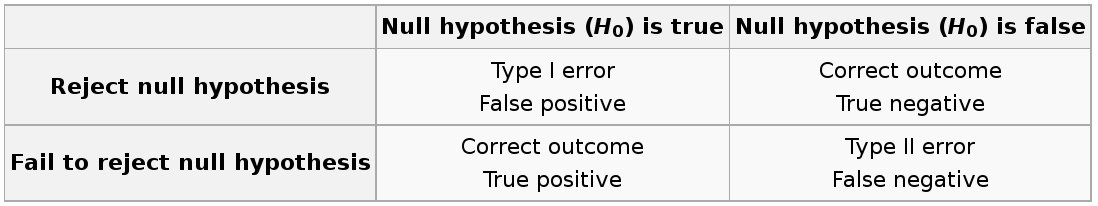
\includegraphics[scale=0.35]{./08_error_kinds.png}
 % 08_error_kinds.png: 1098x206 pixel, 96dpi, 29.05x5.45 cm, bb=0 0 823 154
\end{center}


\end{frame}

\begin{frame}{Test about mean value (normal, known $\sigma$)}
 Sample $\{X_i\}$ of size $n$ from normal distribution $N(\mu, \sigma^2)$, \blue{$\sigma$ known}.
 Statistic (\df{$Z$-test}): 
 \[ Z = \frac{\ol{X} - \mu_0}{\sigma} \sqrt{n} \text{ with distribution $N(0,1)$} \]
 
 \xskip
 \blue{Example:} Reading test in CR: mean 124 points, deviation 12 points. One school, 
 sample of 55 students, we observe sample mean $120$ points.\\
 Is it $95\%$ significant?
 
 \xskip
 $H_0: \mu = 124$, $H_A: \mu < 124$
 
 \xskip
 Critical region: $Z< Z_{crit} <u(0.05) = -1.64$
 
 \[Z=\frac{120 - 124}{12}\sqrt{55} = -2.47\]
 \dots reject hypothesis
\end{frame}


\begin{frame}{$p$-value test \cz{čistý test významnosti}}

\df{ p-value}: smallest level $\alpha$ on which we can reject $H_0$

\xskip
\blue{Our example:} $F_{N(0,1)} ( -2.47 ) = 0.0068$
\end{frame}

\begin{frame}{Comparison of classical and $p$-value $Z$-tests} 

\blue{$H_A: \mu < \mu_0$} $\quad H_0$ rejecting for:
\[ Z_{obs} < u(\alpha) = F^{-1}_{N(0,1)} (\alpha) \quad \text{resp.}\]
\[ p=F(Z_{obs}) <\alpha \]

\xskip
\blue{$H_A: \mu > \mu_0$} $\quad H_0$ rejecting for:
\[ Z_{obs} > u(1-\alpha) = F^{-1}_Z (1-\alpha) \quad \text{resp.}\]
\[ p=1-F(Z_{obs}) <\alpha\]

\xskip
\blue{$H_A: \mu \ne \mu_0$} $\quad H_0$ rejecting for:
\[ Z_{obs} < F^{-1}_Z (\alpha/2) \vee F^{-1}_Z (1-\alpha/2)< Z_{obs} \quad \text{resp.}\]
\[ p= 2\min\{1-F(Z_{obs}) , F(Z_{obs})\} < \alpha\]   
\end{frame}

\begin{frame}{Error of II. kind, reading test example}
Probability $\beta$ of not rejecting $H_0$ for various values of $\mu$. 
\begin{align*}
  1-\beta&=P\left\{ \frac{\ol{X} -\mu_0}{\sigma}\sqrt{n} < u(\alpha)| EX=\mu \right\}\\
  &=P\left\{ \frac{\ol{X} -\mu}{\sigma}\sqrt{n} < \frac{\mu_0-\mu}{\sigma}\sqrt{n}+u(\alpha)| EX=\mu \right\}\\
  &=F_{N(0,1)}\Big(\frac{\mu_0-\mu}{\sigma}\sqrt{n}+u(\alpha) \Big)
\end{align*}
\blue{Example (reading test):}
  $\mu_0=124$, $S_n = 12$, $n=55$, $\alpha=0.05$, $u(\alpha) = -1.64$ \\
  \[
    \beta(\mu)=1-F(\frac{124-\mu}{12}\sqrt{55} - 1.64)
  \]

\end{frame}

\begin{frame}{Error of II. kind, continued}
    \begin{center}
    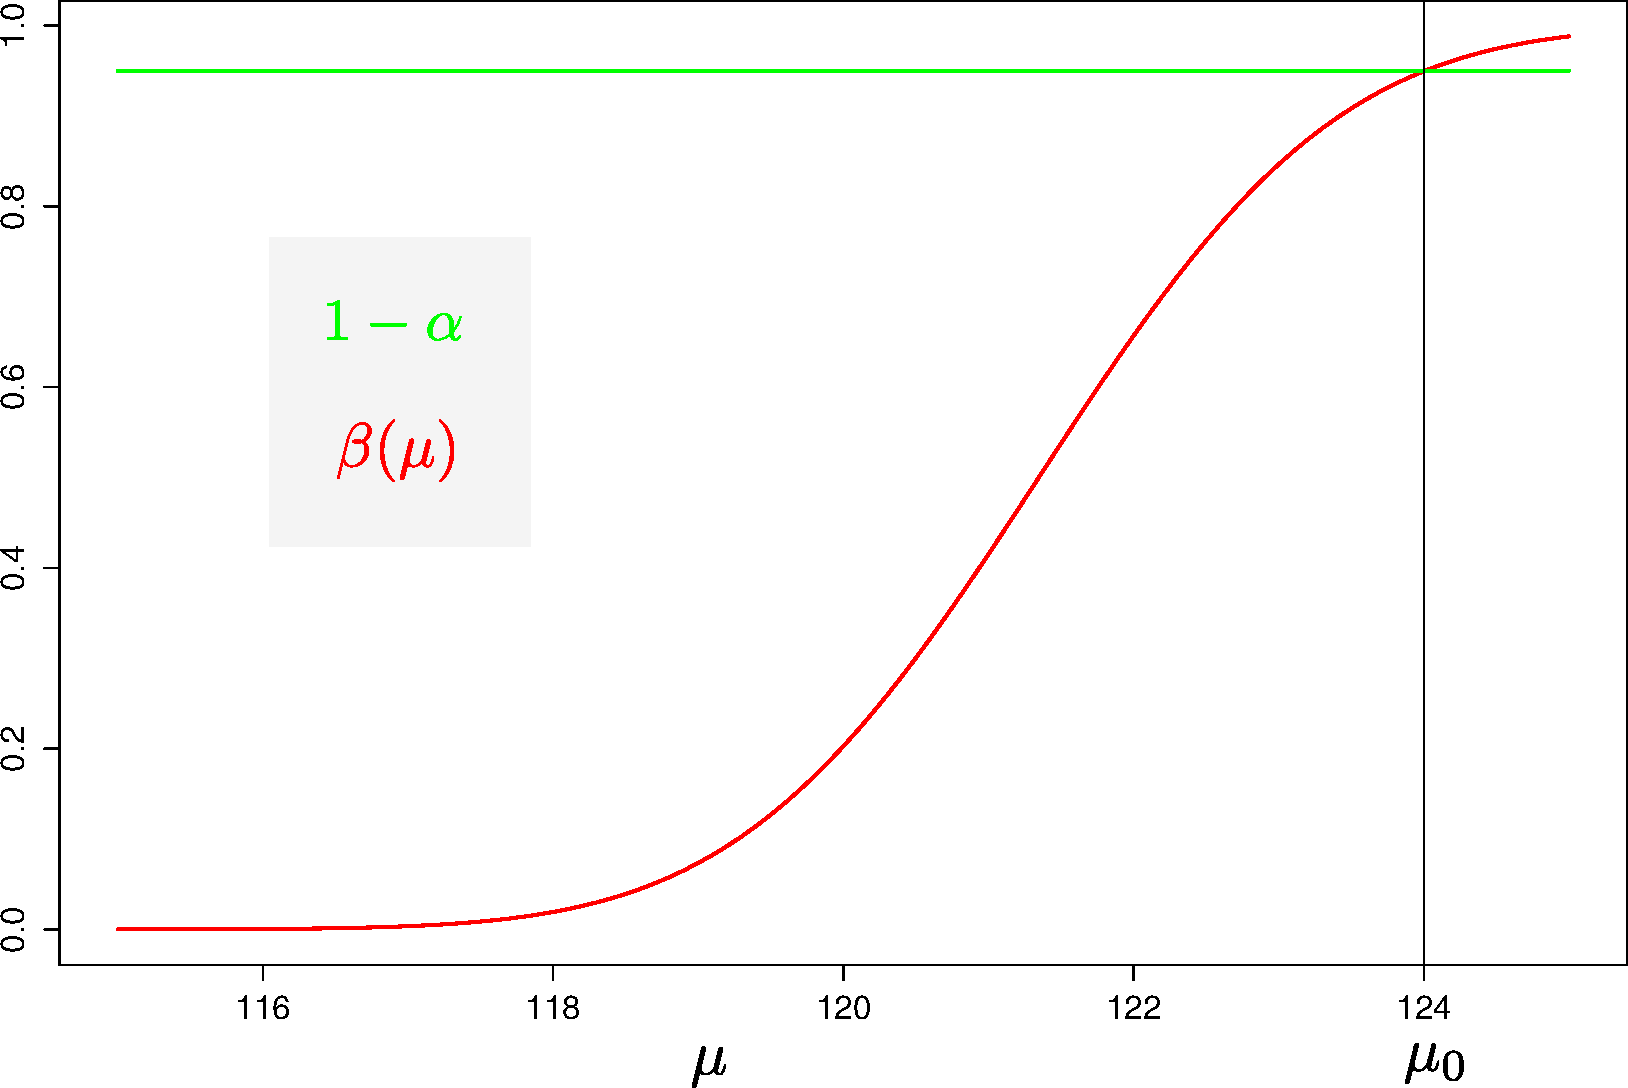
\includegraphics[scale=0.35]{./08_second_error.pdf}
    % 08_error_kinds.png: 1098x206 pixel, 96dpi, 29.05x5.45 cm, bb=0 0 823 154
    \end{center} 
\end{frame}


\begin{frame}[fragile]{Test about mean value (normal, unknown $\sigma$)}
\df{$t$-test}, statistic:
\[
  T = \frac{\ol{X} - \mu_0}{S_n} \sqrt{n} \text{ has Student's distribution } t_{n-1}
\]

\blue{Example:} 
Measurement of heat conductivity coefficient: $0.62$, $0.64$, $0.57$, $0.61$, $0.59$, $0.57$, $0.62$, $0.59$
The nominal coefficient should be $0.60$, decide if there is a significant deviation (assuming normal data).
%data: 0.62, 0.64, 0.57, 0.61, 0.59, 0.57, 0.62, 0.59

\xskip
$H_0$: $\mu = 0.60$, $H_A:$ $\mu\ne 0.60$, two side test

\[
  \ol{X} = 0.60125,\ S_n = 0.02531939,\ T=0.1396,\ p=0.89 
\]
\verb'R> 1-pt(0.1396, 7)    // 0.446454'\\
\verb'R> qt(0.975, 7)       // 2.364624'

\xskip
\dots fail to reject $H_0$.
\end{frame}

\begin{frame}[fragile]{$T$-test in R}
\begin{verbatim}
> hc=c(0.62, 0.64, 0.57, 0.61, 0.59, 0.57, 0.62, 0.59)
> t.test(hc, mu=0.6, conf.level=0.99)

        One Sample t-test

data:  hc 
t = 0.1396, df = 7, p-value = 0.8929
alternative hypothesis: true mean is not equal to 0.6 
99 percent confidence interval:
 0.5699235 0.6325765 
sample estimates:
mean of x 
  0.60125  
\end{verbatim}
\end{frame}




\begin{frame}{Test about variance (or deviation)}
Consider normally distributed sample $X_1, \dots, X_n$.
\[
  X = \frac{S_n^2}{\sigma^2} (n-1) \text{ has $\chi_{n-1}^2$ distribution}
\]

\blue{Example: } Std. deviation in filling beer bottles should not be greater then $0.5$ ml,
Measurement of bottles in liters: $0.4981, 0.5016$, $0.5004, 0.4978$,
$0.4996,0.5002$, $0.4874, 0.4890$, $0.4772, 0.5013, 0.4961$. Is the filling device precise enough?

\xskip
$H_0$: $\sigma = 0.005$, $H_A:$ $\sigma > 0.005$, one side test
$F^{-1}_{\chi^2, 10}(1-0.05) = 18.3$
\[
 S_n = 7.67 ml,\quad \sigma_0 = 5 ml,\quad X=23.55
\]
\dots rejecting $H_0$, $p=1-F(X)=0.009$ 

\xskip
Note: Very sensitive to normality assumption, problematic usage in practice. No dedicated function in R.

\end{frame}



\begin{frame}[fragile]{Test about relative frequency (proportion test)}
sample $X_1,\dots, X_n$ from $Alt(\pi)$, sample relative frequency $p$

\xskip
for $np$ or $n(1-p) > 5$
\[
  T=\frac{p - \pi}{\sqrt{\pi(1-\pi)}}\sqrt{n} \approx N(0,1)
\]
or using F-distribution:
\[
  F_{Bi(n,\pi)}(s) = F_{df_1,df_2} \Big(\frac{df_2(1-\pi)}{df_1\pi}\Big),\ df_1=2(n-s),\ df_2=2(s+1)
\]
\blue{Example:}
$\pi_0 = 0.3, p=0.25, n=50$, $H_A: \pi < \pi_0$

$s=0.25*50=12.5$, $F_{75,25}( 0.84 ) = 0.27$

\dots can not reject for $\alpha <27\%$.

\xskip
{\small
\verb'R> prop.test(0.25*50, n=50, p=0.3, alternative="less", conf.level=0.7)' 
}
\end{frame}





\end{document}


